
%% Article Template
 \documentclass{scrartcl}
 
 %% UTF8 Encoding
 \usepackage[utf8]{inputenc}
 \usepackage[nenglish]{}
 \usepackage[T1]{fontenc}
 \usepackage{lmodern}
 \usepackage{subcaption}
 \usepackage{setspace}
\usepackage{booktabs} % For formal tables`
\usepackage{graphicx}
 
\title{Preliminary Results}
\author{Cédric Milinaire}
\date{Summer period 2019}
\begin{document}

\begin{titlepage}
\maketitle
\end{titlepage} 
 \begin{abstract}
     This document is used to summarize current results. 
 \end{abstract}
\listoffigures
\listoftables
\newpage
 \begin{abstract}
     This document is used to summarize current results. 
 \end{abstract}
\section{Sampling}
For Table \ref{tab:sampling_stats} the text8 dataset was used, all words that occured less than 5 times were deleted from the dataset before each sampling technique.

\begin{table*}[h]\centering
    \caption{Statistics about dataset with different sampling techniques}
    %\scriptsize
    \begin{tabular}{l r r r r}%
        \toprule
      &    \textbf{w/o sampling} & \textbf{Online Sampling} & \textbf{Mikolov} & \textbf{w/o outliers}  \\%
        \midrule%
        Min     &   34 & 34 & 34 & \\%
       Max    & 9Mio & 0.36 Mio. & 0.36 Mio & \\%
      	QTR1      & 79 & 79 & 79\\%
         Median &166 & 166 & 166 & \\%
         Mean & 2227 & 1125 & 1125 & \\%
       QTR3     & 533 & 533 & 534 & \\%
       QTR3 + 1.5IQR   & 1214 & 1214 & 1217  \\%
        \bottomrule%
   \end{tabular}%
   \label{tab:stats_pairs}%
\end{table*}
\begin{table*}[h]\centering
    \caption{Statistics about dataset with different sampling techniques}
    %\scriptsize
    \begin{tabular}{l r r r r}%
        \toprule
      &    \textbf{w/o sampling} & \textbf{Online Sampling} & \textbf{Mikolov} & \textbf{w/o outliers}  \\%
        \midrule%
        Size of Ds   (in words)     &  17 Mio.& 17 Mio. & 8 Mio.& \\%
        Number of Pairs       & 141 Mio. & 71 Mio. & 71. Mio & \\%
        Number of Sentences         & 0.8 Mio & 0.8 Mio & 0.4 Mio  \\%
        \bottomrule%
   \end{tabular}%
   \label{tab:sampling_stats}%
\end{table*}
\newpage

\section{ Boxplots}
\begin{figure}[h!]
\caption{Distribution of the number of pairs per context word without sampling}
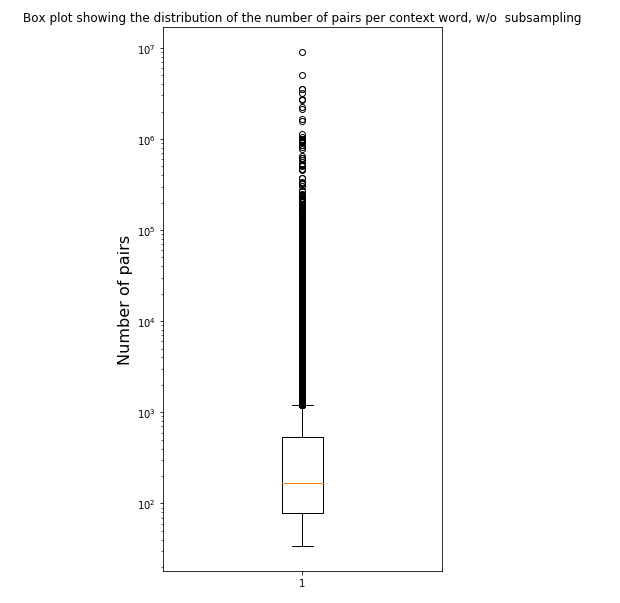
\includegraphics[scale=0.4]{no_sampling_boxplot}
\centering
\end{figure}

\begin{figure}[h!]
\caption{Distribution of the number of pairs per context word with online sampling}
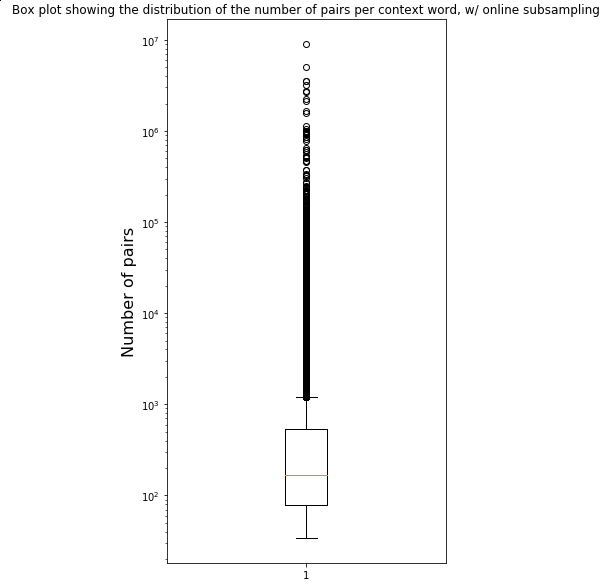
\includegraphics[scale=0.4]{online_sampling_boxplot}
\centering
\end{figure}

\begin{figure}[h!]
\caption{Distribution of the number of pairs per context word with preprocessing sampling}
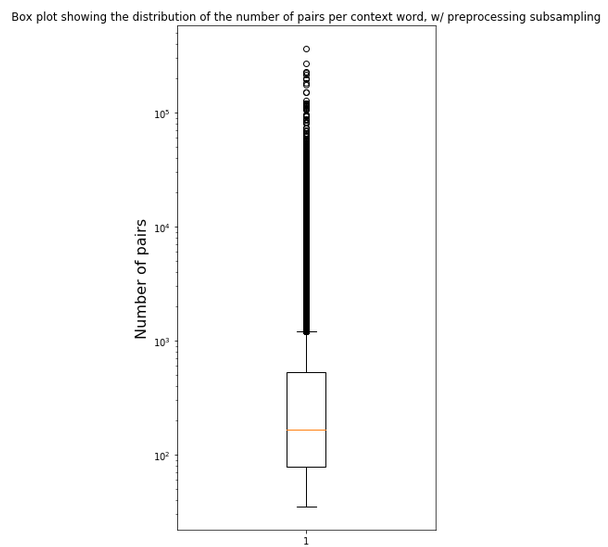
\includegraphics[scale=0.45]{preprocessing_sampling_boxplot}
\centering
\end{figure}

\newpage
\section{Batch\_size}
This section shows a plot of the batch size per batch.
\begin{figure}[h!]
\caption{Batch size per batch}
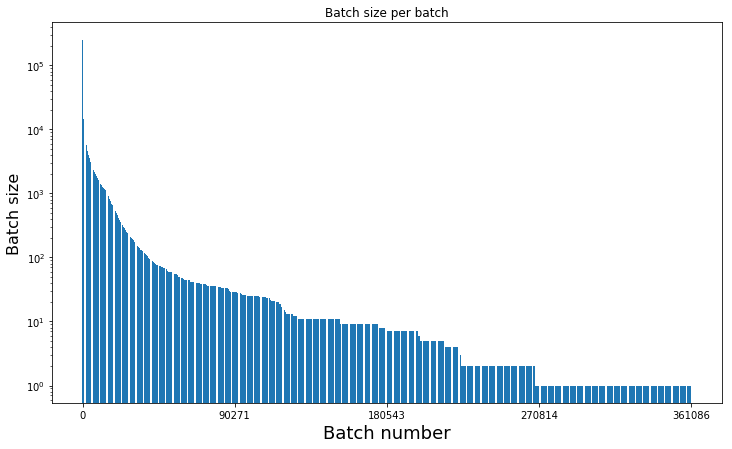
\includegraphics[scale=0.65]{batch_sizes}
\centering
\end{figure}
\section{Results}
Figure shows the results of the training of the text8 dataset without outliers. 
\begin{figure}[h!]
\caption{Results text8 without outliers}
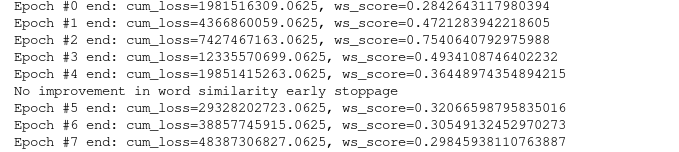
\includegraphics[scale=0.65]{text8_without_outliers}
\centering
\end{figure}


\end{document}

